% Ubah kalimat sesuai dengan judul dari bab ini
\chapter{DESAIN DAN IMPLEMENTASI}

% Ubah konten-konten berikut sesuai dengan yang ingin diisi pada bab ini

\section{Deskripsi Sistem}

Sistem kami bernama JagaBersama, suatu sistem yang dapat digunakan untuk mendeteksi kekerasan baik itu merupakan kekerasan dalam rumah tangga maupun \textit{bullying} atau perundungan yang biasa terjadi di sekolah - sekolah maupun di tempat umum. Dengan memanfaatkan salah satu cabang dalam pembelajaran mesin yaitu \textit{Deep Learning} ditambah dengan pengolahan citra modern, kita dapat melakukan pendeteksian secara otomatis dengan cepat dan murah. Diharapkan dengan adanya sistem kami maka dapat mengurangi jumlah kasus kekerasan di Indonesia dan dapat memberikan suatu ide pendekatan yang baru dalam menanggulangi kekerasan di Indonesia.

Terdapat 2 target pengguna dalam sistem kami, yang pertama adalah Pengguna Umum yang akan memasang sistem kami (kamera + \textit{raspberry pi}) yang akan dapat secara otomatis mendeteksi kekerasan. Kemudian target pengguna yang pertama adalah Agen, agen disini yang dimaksud adalah agen yang dapat berasal dari Komnas Perempuan yang bertugas untuk menyelesaikan apabila terjadi suatu kasus kekerasan maupun bisa juga agen lain seperti polisi atau guru apabila kekerasan terjadi di sekolah.

Namun, sebagai catatan, tanggung jawab saya kebanyakan merupakan pada bagian membuat aplikasi Android yang digunakan sebagai antar-muka antar agen dengan sistem basis data secara keseluruhan.

Seluruh kode yang digunakan untuk melakukan implementasi pada projek ini dapat diakses pada tautan \url{https://github.com/A0040325/capstone_app} untuk implementasi pada bagian aplikasi Android, tautan \url{https://github.com/A0040325/capstone_cloud} untuk implementasi pada bagian \textit{Cloud} dan \textit{Server}, dan tautan \url{https://github.com/A0040325/capstone_ml} untuk implementasi pada bagian pembelajaran mesin. Keseluruhan projek dapat diakses oleh publik secara gratis dan tanpa batasan apapun.

\section{Implementasi Alat}

Terdapat 3 bagian terpisah dari sistem kami yang semuanya bekerja secara bersamaan sehingga menciptakan suatu sistem yang dapat berjalan dengan lancar dan \textit{reliable}. Bagian pertama adalah bagian \textit{Internet of Things} (IoT), selanjutnya adalah \textit{server} sebagai bagian paling penting dalam keseluruhan sistem dan terakhir adalah aplikasi Android sebagai antar-muka dengan agen. Gambar \ref{fig:framework} adalah gambaran secara luas bagaimana sistem kami bekeja secara keseluruhan.


\begin{figure} [!ht]
  \centering
  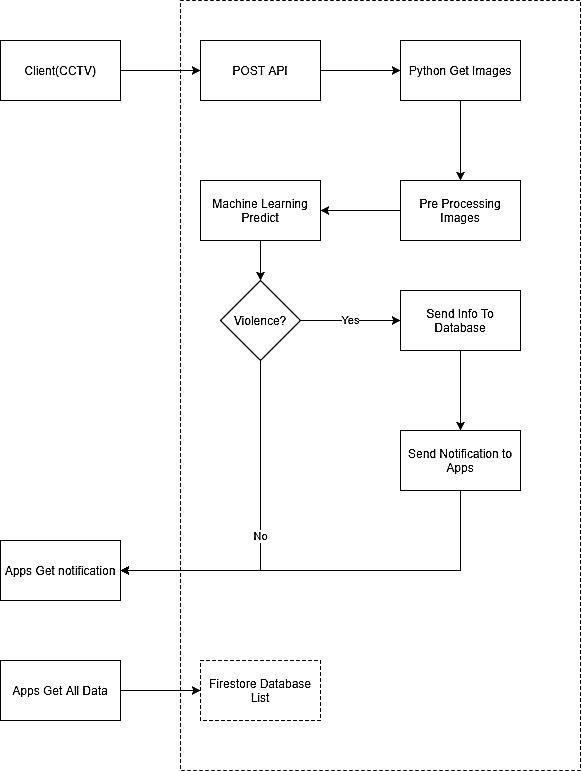
\includegraphics[width=0.8\textwidth]{gambar/framework.jpg}
  % Keterangan gambar yang diinputkan
  \caption{Diagram \textit{Framework} Keseluruhan Proyek}
  % Label referensi dari gambar yang diinputkan
  \label{fig:framework}
\end{figure}

\subsection{Implementasi IoT}

Dalam proyek ini kami berencana untuk menggunakan 2 tipe alat, yang pertama adalah menggunakan CCTV ditambah dengan Raspberry Pi, yang kedua adalah menggunakan CCTV ditambah dengan Jetson Nano yang notabene lebih mahal dibanding alat pertama. Alasan kami memiliki 2 alat adalah kami ingin memberikan pengguna suatu pilihan. Apabila menggunakan Raspberry Pi maka nantinya Raspberry Pi akan mengirimkan foto ke \textit{server} kami setiap beberapa detik sekali sehingga dari sisi \textit{privacy}, hal ini cukup mengkhawatirkan karena walaupun \textit{server} kami sama sekali tidak menyimpan foto dalam jangka waktu yang lama kecuali apbaila dalam foto tersebut terdeteksi adanya kekerasan, namun seseorang dapat melancarkan \textit{Man in The Middle Attack} (MITM), yang berarti seseorang 'menguping' seluruh permintaan koneksi dari \textit{server} ke Raspberry Pi. Alat kedua memiliki tingkat \textit{privacy} yang lebih baik, karena Jetson Nano memiliki kemampuan untuk melakukan deteksi secara \textit{on-device} sehingga hanya mengirimkan data atau foto apabila terdapat kekerasan terdeteksi, namun memerlukan biaya pemasangan yang lebih tinggi.

\subsection{Implementasi \textit{Cloud / Server}}

\textit{Cloud} atau \textit{Server} merupakan salah satu komponen yang paling penting dalam projek kami, selain sebagai tempat menyimpan data, \textit{server} juga digunakan sebagai media pemroses foto yang dikirimkan oleh Raspberry Pi setiap beberapa detik sekali. Sebagai media pemrosesan kami memilih untuk menggunakan App Engine, karena salah satu fitur utamanya yaitu \textit{serverless setup} sehingga kami hanya perlu menyiapkan kode untuk pendeteksi fotonya saja menggunakan teknik pembelajaran mesin.

Untuk teknik pembelajaran mesinnya kami menggunakan teknik \textit{3D Convolutional Neural Network} (3D-CNN), sebuah teknik yang merupakan pengembangan dari CNN biasa dengan cara menambahkan kemampuan untuk melihat tidak secara 1 \textit{frame} atau gambar, melainkan beberapa \textit{frame} sekaligus sehingga sangat cocok digunakan untuk tipe data video yang bersifat sekuensial seperti misalnya untuk mendeteksi orang terjatuh, mendeteksi orang berkelahi sampai mendeteksi kekerasan.

Semua itu kami gabungkan dengan Flask sebagai \textit{webserver} dengan bahasa Python sehingga memudahkan saat implementasi karena hanya memerlukan 1 bahasa saja. Flask kami gunakan sebagai \textit{endpoint} yang dapat diakses oleh Raspberry Pi untuk mengirimkan potongan video setiap beberapa detik sekali.

\begin{figure} [!ht]
  \centering
  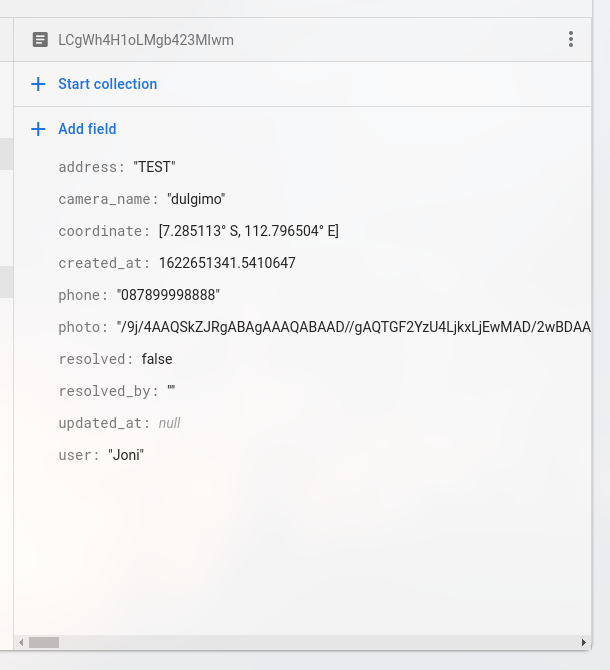
\includegraphics[width=.9\textwidth]{gambar/firestore.png}
  % Keterangan gambar yang diinputkan
  \caption{Implementasi Basis Data}

  \label{fig:db_impl}
\end{figure}

Sebagai media penyimpanan, kami memutuskan untuk menggunakan Firebase, selain karena fiturnya yang lengkap, Firebase sudah menyediakan SDK baik untuk perangkat Android maupun untuk Python sehingga sangat mempermudah dalam melakukan pengembangan sistem. Gambar \ref{fig:db_impl} adalah struktur basis data yang kami gunakan. Terdapat beberapa isian dengan rincian sebagai berikut :

\begin{itemize}
  \item \textit{address}

        Menyimpan data alamat pengguna tempat sistem kami dipasang dan dijalankan. Nilai ini didapat pada saat pemasangan karena setiap alat dari kami sudah memiliki nilai identifikasi masing - masing sehingga memudahkan untuk melakukan pengecekan maupun untuk mengetahui dari kamera mana kekerasan terdeteksi.

  \item \textit{camera\_name}

        Menyimpan nomor identifikasi kamera, berguna untuk mengetahui dari kamera mana foto yang terdeteksi tersebut berasal.

  \item \textit{coordinate}

        Menyimpan data koordinat tempat kekerasan terjadi. Nilai ini didapat dari sistem melalui pengaturan pada saat pemasangan. Fungsi koordinat ini adalah sebagai informasi tambahan dari isian \textit{address} yang sudah disebutkan sebelumnya. Selain itu juga sebagai sumber data yang digunakan untuk menampilkan peta.

  \item \textit{created\_at}

        Menyimpan waktu kapan data dimasukkan ke dalam basis data.

  \item \textit{phone}

        Menyimpan informasi berupa nomor telepon pengguna yang memasang sistem kami. Seperti nilai koordinat, \textit{camera\_name} dan \textit{address}, nilai dari \textit{phone} ini nantinya akan diatur pada saat memasang sistem kami pertama kali.

  \item \textit{photo}

        Adalah isian yang digunakan untuk menyimpan foto yang menunjukkan gambar ketika terjadinya kekerasan. Berformat \textit{base64}  untuk memudahkan dalam menyimpan data sekaligus mengurangi penggunaan media penyimpanan.

  \item \textit{resolved}

        Merupakan penanda apakah suatu kasus statusnya sudah selesai atau masih dalam pengerjaan. Apabila nilai dari isian ini sudah berisi \textit{True}, maka berarti kasus ini sudah selesai dan dimasukkan ke dalam \textit{history}, begitu juga sebaliknya, apabila nilai masih berisi \textit{False}, maka kasus belum selesai dan masih menunggu untuk ditangani.

  \item \textit{resolved\_by}

        Digunakan untuk menyimpan nomor identifikasi agen yang menyelesaikan kasus tersebut, aplikasi menggunakan nilai dari \textit{resolved\_by} dan status \textit{resolved} sebelum memutuskan bahwa kasus sudah selesai dan dimasukkan ke dalam \textit{history}. Apabila status \textit{resolved} masih berisi \textit{False} namun \textit{resolved\_by} sudah memiliki isi, berarti kasus sedang dalam tahap pengerjaan oleh agen yang nomor identifikasinya tersimpan di isian ini.

  \item \textit{updated\_at}

        Menyimpan data tentang kapan suatu kasus mengalami pembaruan, bisa berarti perubahan status kasus yang awalnya \textit{False} menjadi \textit{True} atau perubahan agen yang mengerjakan kasus tersebut. Selain itu dapat juga digunakan untuk mengetahui kapan kasus diselesaikan.

  \item \textit{user}

        Berguna untuk menyimpan nama pengguna yang memasang sistem kami. Seperti data nomor telepon dan beberapa data lainnya, nilai ini diatur pada saat melakukan pemasangan pertama kali.

\end{itemize}

\subsection{Implementasi Aplikasi}

Aplikasi disini digunakan sebagai antar-muka antara agen dengan sistem basis data yang digunakan pada sistem kami. Hal yang pertama kami lakukan adalah melakukan implementasi pada bagian tampilan, disini target utama kami adalah membuat tampilan yang mudah dipahami, serta gampang untuk digunakan.

Gambar \ref{fig:splash_impl} adalah tampilan pada halaman \textit{splash}. \textit{Splash} disini berguna selain untuk melakukan inisialisasi basis data untuk melihat apakah pengguna sudah melakukan \textit{login} sebelumnya, juga digunakan untuk membuat aplikasi tampak lebih cepat dalam dijalankan.

\begin{figure} [!ht]
  \centering
  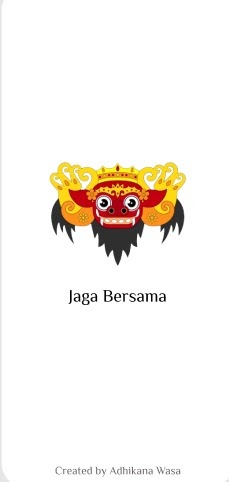
\includegraphics[width=0.5\textwidth]{gambar/splash.jpg}
  % Keterangan gambar yang diinputkan
  \caption{Implementasi Desain \textit{Splash Screen}}
  \label{fig:splash_impl}
\end{figure}

Gambar \ref{fig:login_impl} adalah tampilan pada halaman \textit{sign in}. Tampilan ini adalah yang kedua dilihat setelah memasuki halaman \textit{splash}. Dimana pengguna dapat melakukan \textit{login} untuk mengakses fitur aplikasi lebih lanjut lagi.

\begin{figure} [!ht]
  \centering
  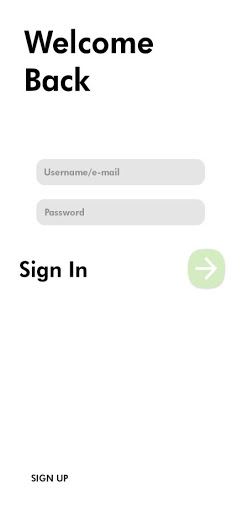
\includegraphics[width=0.5\textwidth]{gambar/signin.jpg}
  % Keterangan gambar yang diinputkan
  \caption{Implementasi Desain Halaman \textit{Sign In}}
  % Label referensi dari gambar yang diinputkan
  \label{fig:login_impl}
\end{figure}

Gambar \ref{fig:signup_impl} adalah tampilan pada halaman \textit{sign up}. Tampilan ini adalah halaman yang akan dilihat saat suatu agen akan membuat akun baru. Terdapat beberapa \textit{field} yang harus diisi apabila akan mendaftar akun baru, yaitu \textit{username}, \textit{email}, nomor telepon dan \textit{password}. \textit{Username}, surel dan \textit{password} digunakan sebagai cara untuk melakukan \textit{login}.

\begin{figure} [!ht]
  \centering
  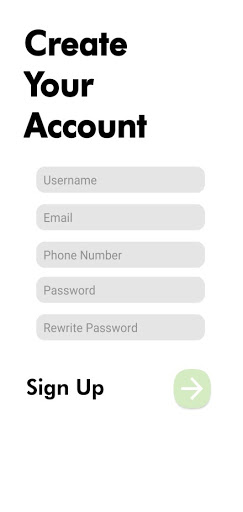
\includegraphics[width=0.5\textwidth]{gambar/signup.jpg}
  % Keterangan gambar yang diinputkan
  \caption{Implementasi Desain Halaman \textit{Sign Up}}
  % Label referensi dari gambar yang diinputkan
  \label{fig:signup_impl}
\end{figure}

Untuk membantu dalam hal melakukan autentikasi, kami menggunakan Firebase Authentication. Firebase Authentication ini dipilih karena selain lebih mudah digunakan dan sudah memiliki fitur keamanan yang cukup. Seperti bisa dilihat pada gambar \ref{fig:auth_db}, kode sandi yang dimasukkan ke dalam basis data akan secara otomatis dilakukan proses enkripsi sehingga data yang dimasukkan menjadi lebih aman dan hanya pengguna sajalah yang tahu apa kode sandi yang digunakan.

\begin{figure} [!ht]
  \centering
  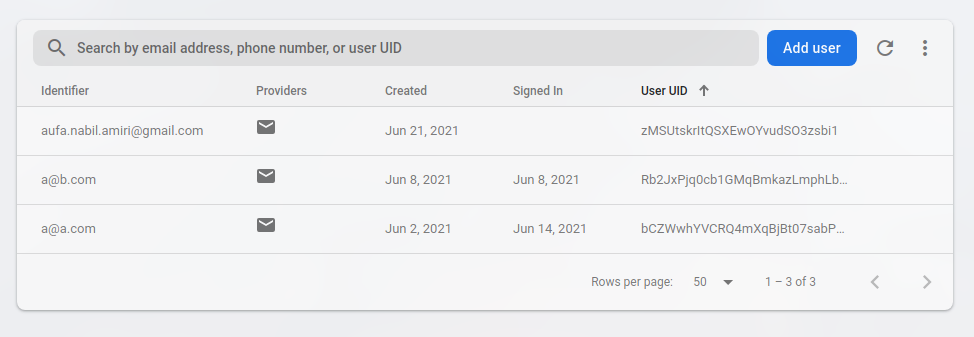
\includegraphics[width=\textwidth]{gambar/firebaseauth.png}
  % Keterangan gambar yang diinputkan
  \caption{Implementasi Autentikasi pada Basis Data}
  % Label referensi dari gambar yang diinputkan
  \label{fig:auth_db}
\end{figure}


Gambar \ref{fig:list_impl} adalah tampilan yang akan paling sering dilihat oleh agen pada saat menggunakan aplikasi yang kami buat, dengan kata lain, halaman ini adalah halaman utama aplikasi kami. Halaman utama ini digunakan untuk melakukan daftar berbagai kasus kekerasan yang belum selesai atau belum ditangani. Nantinya, apabila agen sudah setuju untuk menangani, maka agen hanya perlu menekan tombol 'TERIMA', sistem akan otomatis mencatat nama agen tersebut sebagai agen yang datang ke lokasi dan menyelesaikan kasus kekerasan yang terjadi. Saat kasus sudah selesai, maka agen harus menekan tombol 'SELESAI' pada daftar kasus di aplikasi, dengan menekan tombol tersebut, maka kasus akan dinyatakan selesai dan masuk ke dalam \textit{history} kasus.

\begin{figure} [!ht]
  \centering
  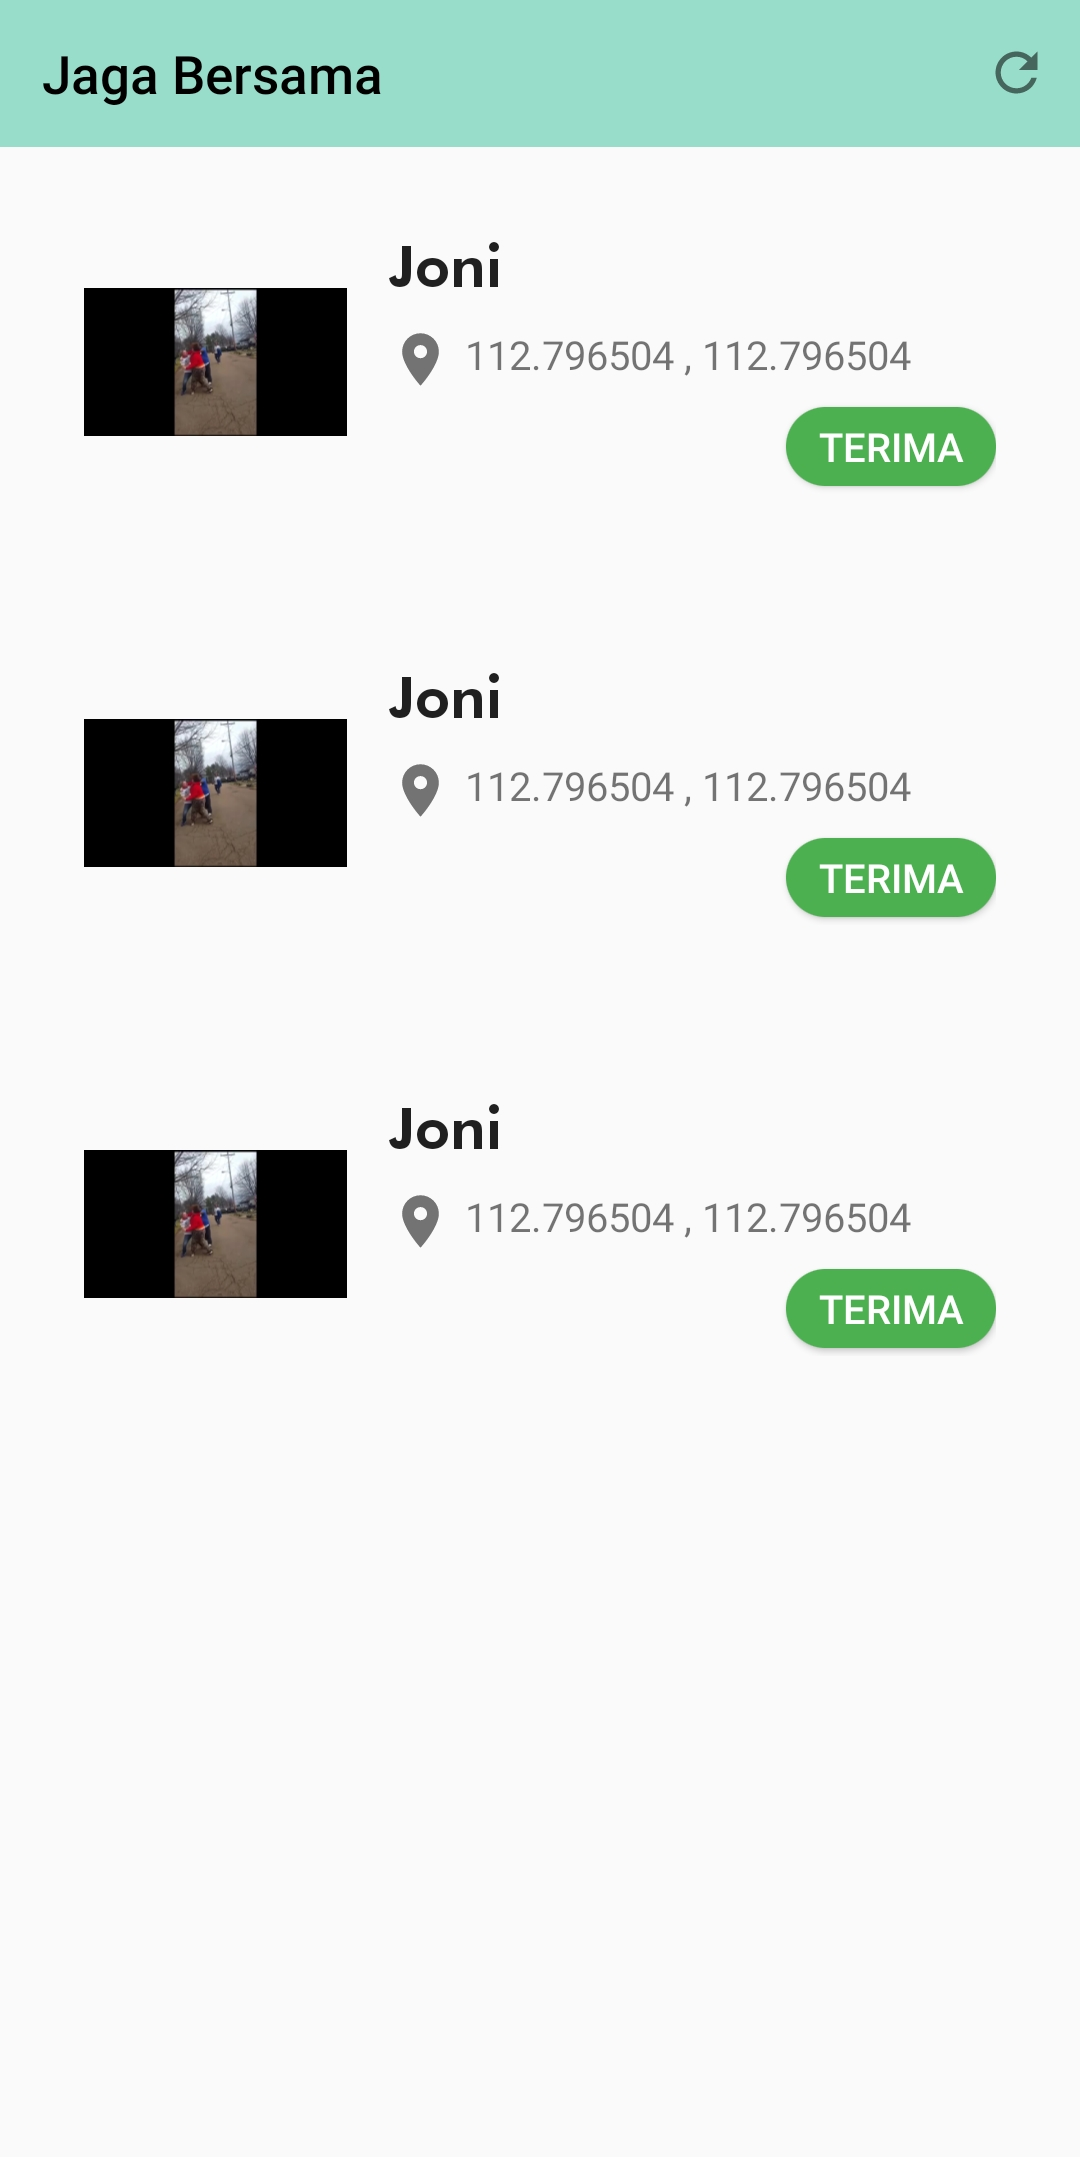
\includegraphics[width=0.5\textwidth]{gambar/list.jpeg}
  % Keterangan gambar yang diinputkan
  \caption{Implementasi Desain Halaman Daftar Kekerasan yang Belum Selesai}
  % Label referensi dari gambar yang diinputkan
  \label{fig:list_impl}
\end{figure}

Apabila agen menekan pada bagian tengah pada daftar kekerasan, maka halaman akan berpindah ke halaman detail. Gambar \ref{fig:detail_impl} adalah tampilan dari halaman detail. Halaman detail ini digunakan untuk menunjukkan detail dari kekerasan, terdapat beberapa data diantaranya adalah foto kekerasan yang terjadi, data lengkap pengguna, tampilan peta tempat lokasi kejadian dan tombol untuk melakukan panggilan dengan mudah karena hanya memerlukan 1 kali menekan tombol tersebut saja.

\begin{figure} [!ht]
  \centering
  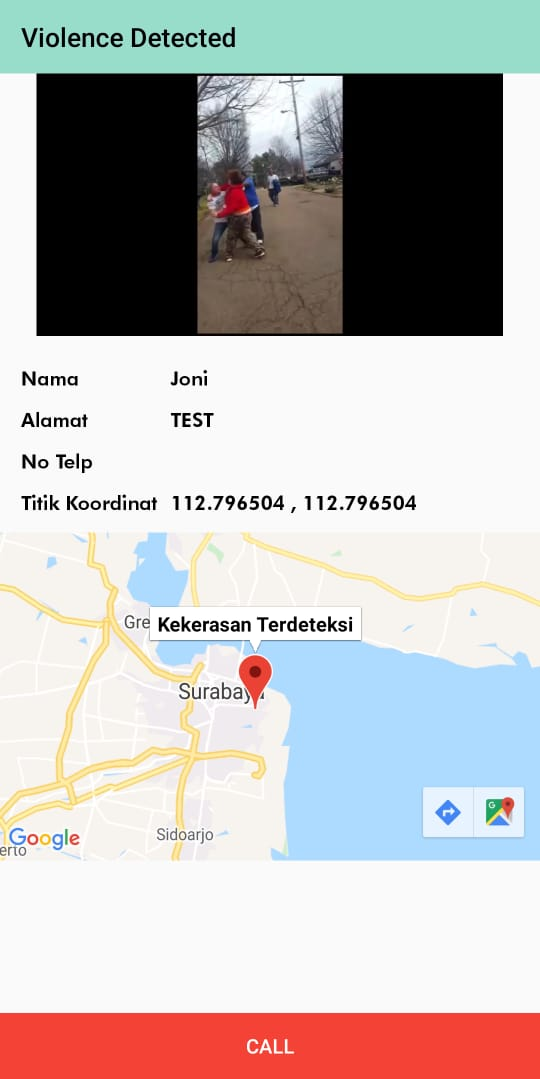
\includegraphics[width=0.5\textwidth]{gambar/detail.jpeg}
  % Keterangan gambar yang diinputkan
  \caption{Implementasi Desain Halaman Detail Kekerasan}
  % Label referensi dari gambar yang diinputkan
  \label{fig:detail_impl}
\end{figure}